\chapter{Intrinsic Properties and Scattering Mechanisms}\label{chap:results}
At present, much of the problems that remain in the \acs{TMD} and heterostructure community are centered around the improvement of device performance and determining the limiting factors of such devices. As such, in order to overcome these hurdles some new innovative techniques have been introduced. One of these is the problem of making quality metal/semiconductor contacts, several approaches exist for attempting to reconcile this, however, the approaches do not seem to be universal for all types of \acp{TMD}. Coming up with a solution to this problem ultimately allows for the further understanding of some of the other remaining problems, such as device mobility limits. This has been of much debate in the community and first principles calculations predict values higher than what has so far been reported experimentally, suggesting room for improvements. To improve mobility, it must first be understood what factors limit the mobility. However, to do this the contact resistance must be low otherwise one cannot examine the intrinsic channel properties with high-resistance contacts. Ultimately, these concerns and their solutions are fueled by the desire feasibility in device applications. This aspect leads to another factor of concern, how doping effects the mobility and device performance. Inventing novel approaches to these problems will, in the future, lead to better \acs{TMD} devices and eventual applications.

\section{Approach to Low-Resistance Contacts}\label{sec:contacts}
Developing low-resistance contacts is important two enable the study of intrinsic transport properties of devices, but also it is vital to applications of \acp{TMD}. Large contact resistance at room temperature is not ideal for applications. At the metal/semiconductor contact interface a barrier develops, the \acs{SB} \cite{Schottky_ZPhys1938}. The device in question must be able to supply the necessary current, and the voltage drop across the contacts should be small compared to the voltage drop across the device's active channel region. In most cases, the contacts should be ohmic, the current-voltage characteristic should be linear and not degrade the device's performance to any significant extent \cite{Rideout_Solid1975}. In the ideal, theoretical case (Schottky-Mott model)  the \acs{SBH} is given by 
\begin{equation}\label{eq:schottky_mott}
	\Phi_{\mathrm{B}p} = \frac{E_g}{e}- \left(\Phi_m - \chi_s\right),
\end{equation}
where $\Phi_{\mathrm{B}p}$ is the hole barrier height, $e$ is the charge of an electron, $E_g$ is the semiconductor bandgap energy, $\Phi_m$ is the metal workfunction, $\chi_s$ is the semiconductor electron affinity, note that these properties are intrinsic to the material before forming the junction \cite{Rhoderick_Book1988}. In reality the description is not this simple and is largely dependent on other factors, such as imperfections, Fermi level pinning, and Fermi level mismatch \cite{Cohen_Book2014}. For a metal/$p$-type semiconductor interface the magnitude of the \acs{SBH} is reflective of the mismatch in Fermi level of the metal and the \ac{VBM} of the semiconductor. Conversely, for the case of a metal/$n$-type interface it is the mismatch in the Fermi level of the metal and the \ac{CBM} of the semiconductor \cite{Tung_AppPhysRev2014}. Therefore, to address the issue of contact resistance one must find ways to effectively ``tune" the \acs{SB}.\\ \\

There have been several approaches employed in order to reduce the contact resistance. One method is to attempt to tune the \acs{SBH} by using different common metals to find a desirable work function. Eq.~\ref{eq:schottky_mott} implies that the \acs{SBH} is linearly dependent on the work function $\Phi_m$ of the metal. However, in reality, this is usually not the case because, one, finding metals with the proper work function that minimizes the \acs{SBH} while still maintaining high conductivity has proven to be difficult, and, two, the lowering that would potentially be achieved by the use of the proper work function would most likely be diminished due to Fermi level pinning \cite{Liu_ACSnano2012,Das_NanoLett2012,Liu_arxiv2016}. Fermi level pinning occurs when there are surface states that develop in the bandgap and pin the Fermi level position of the semiconductor \cite{Tung_AppPhysRev2014}. Another method is the use of graphene contacts \cite{HJ_Chuang_NanoLett2014,Das_NanoLett2014,Roy_ACSnano2014}. Barrier-free contacts have been achieved using this method in combination with \ch{MoS2} using a gate potential to tune band alignment \cite{Liu_NanoLett2015}. However, this method has not been shown to be extendable down to low enough contact resistances in some other \acp{TMD}, most notably \ch{WSe2}, but has been shown to be tunable down to $(<2\unita{k\Omega}\unita{\mu m}$) \cite{Chuang_2016,HJ_Chuang_NanoLett2014}. The method to that is enacted here to reduce the contact resistance is using degenerately doped contact regions. By degenerately doping the contact region one can thin the \acs{SB} width. However, this method is not without its challenges as well. Several doping techniques that can be used have limited spatial resolution \cite{Farmanbar_arxiv2016}. Depsite the challenges posed, this method has produced promising results that are transferrable to \acp{TMD} including \ch{WSe2}, \ch{MoS2}, and \ch{MoSe2} resulting in high-performance, low contact resistance devices. \\ \\

To determine the contact resistance of fabricated devices a method known as \ac{TLM} is used. In general, resistance is given by
\begin{equation}\label{eq:resistance_general}
	R = \frac{\rho}{A}l,
\end{equation}
where, in this case, it is assume that the resistivity $\rho$ and the area $A$ of the electrodes are constant throughout the device \cite{Schroder_Semiconductor2006}. The resistance $R$ is then proportional to the length of the channel $l$. By determining the resistance as a function of length one can deduce the contact resistance. The total contact resistance is given by
\begin{equation}\label{eq:contact_r}
	R = R_\mathrm{ch} + 2R_\mathrm{c},
\end{equation} 
where $R_\mathrm{c}$ and $R_\mathrm{ch}$ are the contact and channel resistances, respectively \cite{Schroder_Semiconductor2006}. A typical device for a \acs{TLM} measurement has drain and source electrodes with varying lengths between them. By find the resistance from the gradient of an $IV$ characteristic curve, one can apply the logic from eqs.~\ref{eq:resistance_general} and \ref{eq:contact_r} to find the contact resistance. The contact resistance is ultimately extracted from the $y$-intercept of a linear fit of resistance as a function of length for the device. In general, this method is done at several temperatures to further characterize the quality of the contacts as one would expect that at low temperatures, for low-resistance contacts, they would behave in similar fashion as they did at higher temperatures. To determine the affect that varying doping schemes has on contact resistance devices that were lightly doped (\lightlyfive) were measured using \acs{TLM} and compared to degenerately doped devices (\degenerate).

\subsection{Transmission Line Method: \lightlyfive}\label{subsec:TLM_lightly}
As stated in sec.~\ref{sec:contacts}, the \acs{TLM} measurement involves designing a device that has varying drain source channel lengths in order to determine the resistance as a function of length. Fig.~\subref*{fig:transmission_device_10232015_no1} shows an optical micrograph consisting of a lightly doped \ch{WSe2} (\lightlyfive) channel. Figs.~\subref*{fig:tlm_resistance1}-\subref*{fig:tlm_resistance3} show the total resistance as a function of length for both $V_{bg}=0\unita{V}$ and $V_{bg}=-60\unita{V}$ at room temperature. The contact resistance are then determine from the linear fit and the $y$-intercept. These figures show ohmic contacts with a minimum contact resistance of $R_\mathrm{c}=2.35\unita{k\Omega}\unita{\mu m}$ achieved with application of $V_{bg}=-60\unita{V}$. In addition, the contact resistances are lower for the higher values of $V_{bg}$. This is due, in part, to the fact that the higher $V_{bg}$ works to reduce the width of the \acs{SB} and allow for more transmission across the barrier that has developed between the metal/semiconductor interface. Moreover, when there is no $V_{bg}$ applied, the reported contact resistances are an order of magnitude higher. The fact that the channel material in use here is only lightly doped means that there is a larger mismatch between the Fermi level of the metal and the \acs{VBM} causing a larger \acs{SBH} than one would expect with a channel that was more heavily doped.
\begin{figure}[ht]
	\centering
	\subfloat[]{
		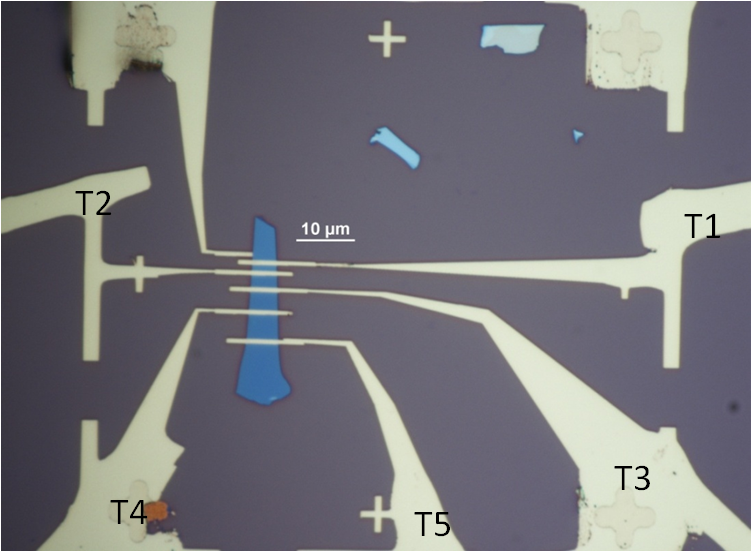
\includegraphics[height=4.25cm,width=5.0cm]{figs/results/transmission_line/transmission_device_pic_5-5_21_10232015_no1}
		\label{fig:transmission_device_10232015_no1}
	}
	\subfloat[]{
		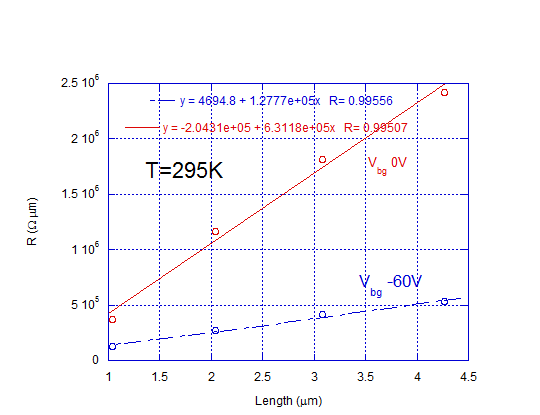
\includegraphics[height=4.25cm,width=5.0cm]{figs/results/transmission_line/transmission_resistance_plot_pic_5-5_21_10232015_no1}
		\label{fig:tlm_resistance1}
	}

	%\qquad
	\subfloat[]{
		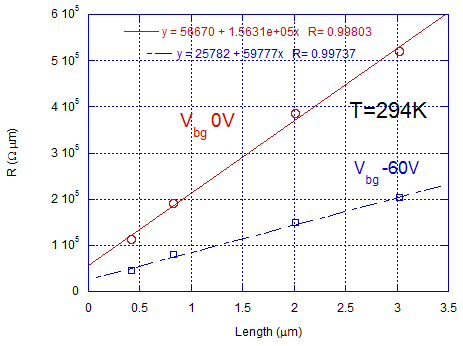
\includegraphics[height=4.25cm,width=5.0cm]{figs/results/transmission_line/transmission_resistance_plot_pic_56_21_10232015_no2}
		\label{fig:tlm_resistance2}
	}
	\subfloat[]{
		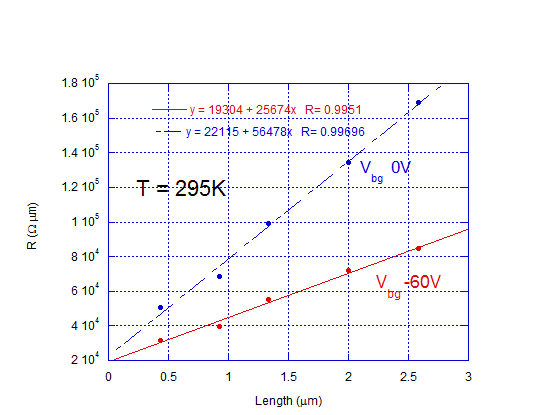
\includegraphics[height=4.25cm,width=5.0cm]{figs/results/transmission_line/transmission_resistance_plot_pic_-66_21_11182015_no2}
		\label{fig:tlm_resistance3}
	}
	\caption[TLM: contact resistances using \lightlyfive]{\protect\subref{fig:transmission_device_10232015_no1} Optical micrograph of a device structure for \acs{TLM} measurement consisting of lightly $p$-doped \ch{WSe2} (\lightlyfive) with \ch{Ti}/\ch{Au} metal contacts. \protect\subref{fig:tlm_resistance1}-\protect\subref{fig:tlm_resistance3} Normalized total resistance as a function of channel length measured at room temperature.}
	\label{fig:tlm_resistance_measurement_lightly}
\end{figure}

\subsection{Transmission Line Method: \degenerate}\label{subsec:TLM_degenerate}
The lightly doped \ch{WSe2} device showed reasonably low contact resistances at room temperature, but lower-resistance contacts are desired. Using \acs{TLM} degenerately doped \ch{WSe2} (\degenerate) devices were measured. Fig.~\subref*{fig:ben_tlm_resistance1} shows an optical micrograph of the device design which identical to that in sec.~\ref{subsec:TLM_lightly}. The contact resistances as a function of length are shown in figs.~\subref*{fig:ben_tlm_resistance2} and \subref*{fig:ben_tlm_resistance3} at room temperature and $5\unita{K}$, respectively. At both temperatures they exhibit linear ohmic behavior. Even more promising is that the values for contact resistance are essentially the same at high and low temperature, which indicates significant reduction of the \acs{SB}. The low temperature performance means that the contacts are of high quality as the contacts tend to degrade as temperature decreases mainly due to the lack of thermionic emmission of carriers \cite{Tung_AppPhysRev2014}. 
\begin{figure}[ht]
	\centering
	\subfloat[]{
		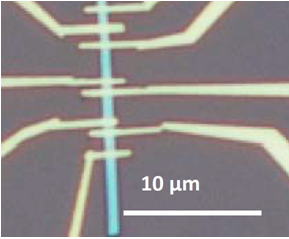
\includegraphics[height=4.25cm,width=5.0cm]{figs/results/transmission_line/ben_tlm_degenerately_doped_device_pic}
		\label{fig:ben_tlm_resistance1}
	}
	%\qquad
	\subfloat[]{
		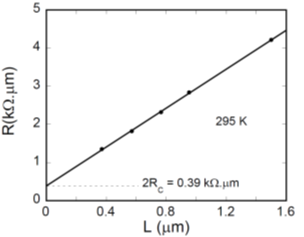
\includegraphics[height=4.25cm,width=5.0cm]{figs/results/transmission_line/ben_tlm_degenerately_doped_resistance_295K}
		\label{fig:ben_tlm_resistance2}
	}
	%\qquad
	\subfloat[]{
		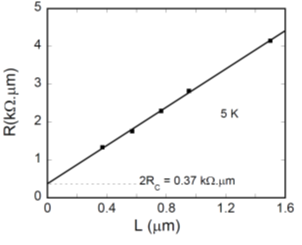
\includegraphics[height=4.25cm,width=5.0cm]{figs/results/transmission_line/ben_tlm_degenerately_doped_resistance_5K}
		\label{fig:ben_tlm_resistance3}
	}
	\caption[TLM: contact resistances using \degenerate]{\protect\subref{fig:ben_tlm_resistance1} Optical micrograph of a device structure for \acs{TLM} measurement consisting of degenerately $p$-doped \ch{WSe2} (\degenerate) with \ch{Ti}/\ch{Au} metal contacts. \protect\subref{fig:ben_tlm_resistance2} Normalized total resistance as a function of channel length measured at room temperature $T=295\unita{K}$ and \protect\subref{fig:ben_tlm_resistance3} low temperature $T=5\unita{K}$. Figures appeared in ref.~\cite{Chuang_2016}.}
	\label{fig:tlm_resistance_measurement_degenerate}
\end{figure}

\subsection{Discussion of Results for Light and Degenerately Doped Contacts}\label{subsec:contact_discussion}
The results for lightly (\lightlyfive) and degenerately (\degenerate) doped \ch{WSe2} contacts are summarized in table~\ref{table:contact_summary}. The degenerately doped contacts have resistances of at least an order of magnitude lower at room temperature due to the lowered \acs{SBH} from the higher doping scheme. The lightly doped contacts, though still relatively high, demonstrate the effect that applying a higher $V_{bg}$ can have on the \acs{SB}. An effective thinning of the barrier is observed for higher backgate voltage and thus this can also be used to further tune the \acs{SB} and lower contact resistances. The results from the lightly doped \ch{WSe2} channel are on the same order of magnitude as what has been previously shown using graphene/\ch{WSe2} contacts ($\sim 2\unita{k\Omega}\unita{\mu m}$) \cite{HJ_Chuang_NanoLett2014}. The results shown obtained for the degenerately doped \ch{WSe2} are significantly lower than graphene/\ch{WSe2} method and are in line with the best results that have been achieved for \acp{TMD} ($\sim 0.2-0.7\unita{k\Omega}\unita{\mu m}$ ) \cite{Yang_NanoLett2014,Kappera_NatureMat2014,Leong_ACSnano2014}. With these results in mind, this 2D/2D contact method using degenerately doped \ch{WSe2} (\degenerate) looks to be a viable and effective way to engineer low-resistance contacts which will be essential to explore the intrinsic channel properties of \acp{TMD}, the performance limits, and also when it comes to applications.
\begin{table}[ht]
	\centering
	\begin{threeparttable}
		\begin{tabular}{c c c}
			%\hline\hline
			\toprule
			Doping Content & Temperature ($\unita{K}$) & $R_\mathrm{c}(\unita{k\Omega}\unita{\mu m})$\tnote{$\ast$} \\ [0.5ex]
			%\hline
			\midrule
			$(0.05\%)$ \lightlyfive & 295 & $2.35$\tnote{$\dagger$}\\
			$(0.05\%)$ \lightlyfive & 294 & $12.9$\tnote{$\dagger$}\\
			$(0.05\%)$ \lightlyfive & 295 & $9.65$\tnote{$\dagger$}\\ 
			$(0.5\%)$ \degenerate & 295 & $0.195$\tnote{$\ddagger$}\\ 
			$(0.5\%)$ \degenerate & 5 & $0.185$\tnote{$\ddagger$}\\[1ex]
			%\hline
			\bottomrule
		\end{tabular}
		\begin{tablenotes}
			\item[$\ast$] The contact resistances $R_\mathrm{c}$ are reported as per electrode by taking the intercept and dividing by 2. In some other references this may not be the case.
			\item[$\dagger$] Resistance values from figs.~\subref*{fig:tlm_resistance1}, \subref*{fig:tlm_resistance2}, and \subref*{fig:tlm_resistance3}.
			\item[$\ddagger$] Resistance values from figs.~\subref*{fig:ben_tlm_resistance2} and \subref*{fig:ben_tlm_resistance3}.
		\end{tablenotes}
	\caption[Summary of contact resistances lightly $p$-doped and degenerately $p$-doped \ch{WSe2}]{Summary of contact resistances for lightly $p$-doped \ch{WSe2} (\lightlyfive) and degenerately $p$-doped \ch{WSe2} (\degenerate) found using linear fit data from figs.~\subref*{fig:tlm_resistance1}-\subref*{fig:tlm_resistance3} and \subref*{fig:ben_tlm_resistance2}-\subref*{fig:ben_tlm_resistance3}.}
	\label{table:contact_summary}
	\end{threeparttable}
\end{table}

\section{Field-Effect Mobility and Scattering Mechanisms}\label{sec:mufe_scatter}
There are several properties to electrically characterize and quantify the performance of a device. One such property is the two-probe and four-probe field-effect mobility $\mu_\mathrm{FE}$. The two-probe field-effect mobility is given by 
\begin{equation}\label{eq:mu_fe2}
	\mu_\mathrm{FE} = \frac{L}{w}\frac{1}{C}\frac{1}{V_{ds}}\frac{d I_{ds}}{V_{bg}},
\end{equation}
where $L$ is the length of the channel (the distance between the source and drain), $w$ is the width of the channel, $I_{ds}$ is the drain current, $V_{bg}$ is the backgate voltage, $V_{ds}$ is the drain voltage, and $C$ is the geometric capacitance \cite{Stassen_AppPhysLett2004}. To measure the field-effect mobility there are two main approaches used, either the two-probe method or the four-probe method. The two-probe method is shown in fig.~\subref*{fig:two_probe}. In this configuration measurement takes place between the drain and source only. The main drawback of this measurement is that it is subject to resistance that can make data difficult to interpret because of this \cite{Schroder_Semiconductor2006}. Alternatively, there is the four-point probe configuration which is shown in fig.~\subref*{fig:four_probe} \cite{Valdes_IRE1954}. The main advantage of this configuration is that the voltage drop is measured across $V_3$ and $V_2$ and therefore allows the resistance to be subtracted. The field-effect mobility is important to characterizing a device because, it can reveal information about scattering mechanisms present and how they affect the mobility. Also, depending on the device's channel and whether it is doped or not, the mobility shows how the doping can be tuned to perform in a desired manner for device applications, especially at room temperature. To begin to study these issues devices with varying doping schemes and fabrication methods were measured to address where improvements can be made and where unknowns still exist.
\begin{figure}[ht]
	\centering
	\subfloat[]{
		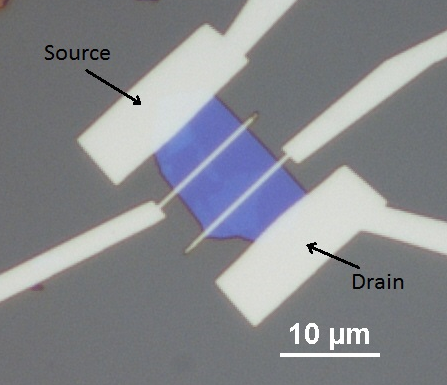
\includegraphics[height=4cm,width=4.75cm]{figs/-44_54_100x_after_liftoff_two_point_probe_measurement}
		\label{fig:two_probe}
	}
	\qquad
	\subfloat[]{
		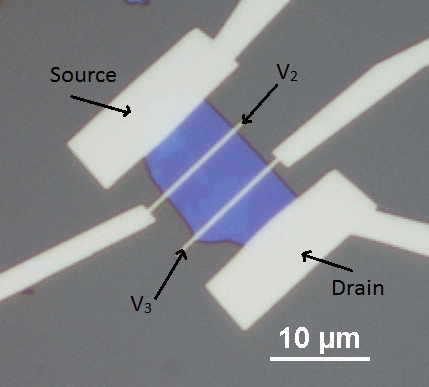
\includegraphics[height=4cm,width=4.75cm]{figs/-44_54_100x_after_liftoff_four_point_measurement}
		\label{fig:four_probe}
	}
	\caption[Field-effect mobility measurement configuration]{Examples of \protect\subref{fig:two_probe} two-point probe measurement configuration for field-effect mobility measurements and \protect\subref{fig:four_probe} four-point probe configuration.}
\end{figure}

\subsection{Applying Low-Resistance Contacts: Doped Channel}\label{subsec:mufe_doped_channel}
It is important to understand the how doping affects the mobility of a device, especially for device applications. To study this, device's with were fabricated using the method outlined in figs.~\ref{fig:pWSe2_doped_contacts_and_channel_step1}-\ref{fig:pWSe2_doped_contacts_and_channel_final_device}. A piece of \hbn is first transferred onto the \ch{Si}/\ch{SiO2} substrate. This is done because \hbn is smoother than the plain \ch{Si}/\ch{SiO2} substrate and acts to reduce and effectively eliminate the majority of substrate and roughness scattering that would be present otherwise. 
\begin{figure}
	\centering
	\subfloat[]{
		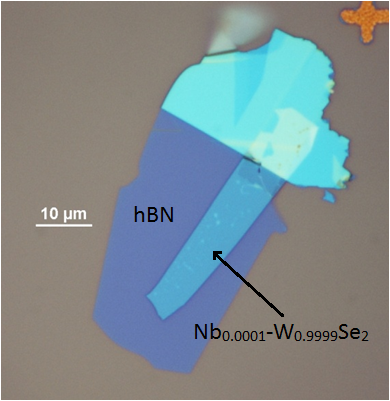
\includegraphics[height=3.75cm,width=3cm]{figs/results/hall_bar_doped_channel_doped_contacts/pWSe2_on_hBN_substrate_5-5_21_no1_annotated}
		\label{fig:pWSe2_doped_contacts_and_channel_step1}
	}
	\qquad
	\subfloat[]{
		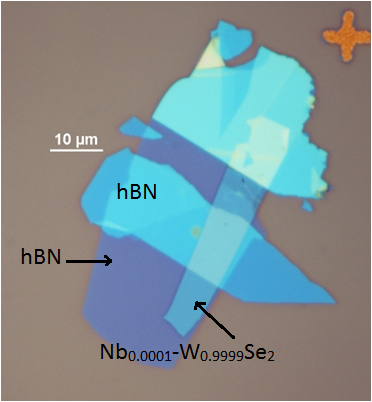
\includegraphics[height=3.75cm,width=3cm]{figs/results/hall_bar_doped_channel_doped_contacts/pWSe2_on_hBN_substrate_with_top_hBN_5-5_21_no1_annotated}
		\label{fig:pWSe2_doped_contacts_and_channel_step2}
	}
	\qquad
	\subfloat[]{
		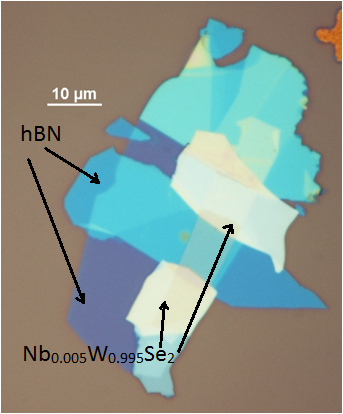
\includegraphics[height=3.75cm,width=3cm]{figs/results/hall_bar_doped_channel_doped_contacts/pWSe2_on_hBN_substrate_with_top_hBN_doped_contact_transfer_5-5_21_no1_annotated}
		\label{fig:pWSe2_doped_contacts_and_channel_step3}
	}
	\qquad
	\subfloat[]{
		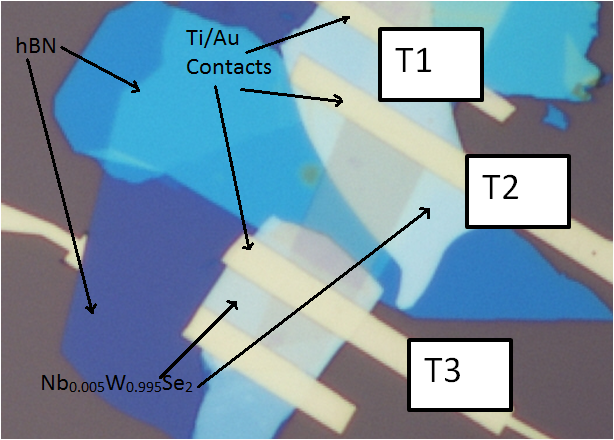
\includegraphics[height=3cm,width=3.75cm]{figs/results/hall_bar_doped_channel_doped_contacts/pWSe2_device_with_electrodes_5-5_21_no1_annotated}
		\label{fig:pWSe2_doped_contacts_and_channel_final_device}
	}
	\caption[Fabrication steps of \lightlyone channel with \degenerate\, contacts]{\protect\subref{fig:pWSe2_doped_contacts_and_channel_step1} \lightlyone transferred to \hbn substate,  \protect\subref{fig:pWSe2_doped_contacts_and_channel_step2} top \hbn transferred onto channel, \protect\subref{fig:pWSe2_doped_contacts_and_channel_step3} degenerately doped (\degenerate) contacts transferred onto device, and \protect\subref{fig:pWSe2_doped_contacts_and_channel_final_device} device after fabrication steps with \ch{Ti}/\ch{Au} metal electrodes consisting of a $5.6\unita{nm}$ thick channel.}
	\label{fig:hBN_field_effect_device_fab}
\end{figure}
Next, the channel is transferred onto the \hbn substrate, in this case \lightlyone (fig.~\ref{fig:pWSe2_doped_contacts_and_channel_step1}). This is followed by another piece of \hbn which acts to cover the channel and protect it from external effects (fig.~\ref{fig:pWSe2_doped_contacts_and_channel_step2}). The degenerately doped contacts are added and cover the remaining exposed pieces of the channel for the reasons outlined in sec.~\ref{sec:contacts} (fig.~\ref{fig:pWSe2_doped_contacts_and_channel_step3}). Electrodes are fabricated on the device in order to perform a two-probe measurement (fig.~\ref{fig:pWSe2_doped_contacts_and_channel_final_device}). 

The device was characterized first without annealing the device. Figs.~\ref{fig:5-5_21_no1_pre_anneal_iv_300k} and \ref{fig:5-5_21_no1_pre_anneal_iv_10k} show the $IV$ characteristic curves at $T=300\unita{K}$ and $T=10\unita{K}$, respectively. Ohmic contacts are observed at high temperature, however, at low temperature the curve becomes nonlinear indicating a non-ohmic behavior. Additionally, fig.~\ref{fig:5-5_21_no1_pre_anneal_mu_fe_vs_temp} shows the field-effect mobility as a function of temperature. The behavior is that of increasing mobility with decreasing temperature, however, there is a deviation in the mobility for $V_{ds} = -50\unita{mV}$ as compared to $V_{ds} = -1\unita{V}$ at low temperatures. One would expect the two curves to be relatively identical. 
\begin{figure}[ht]
	\centering 
	\subfloat[]{
		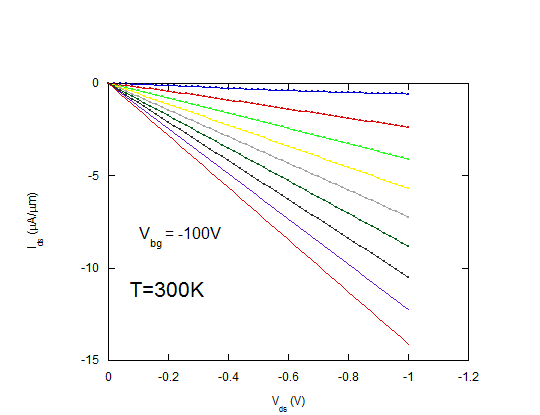
\includegraphics[height=4.55cm,width=5.3cm]{figs/results/hall_bar_doped_channel_doped_contacts/Vds-Id_Vds_1V_-1V-Vbg_-20V_-100V_T2-T3_300K-04_plot_before_anneal_5-5_21_no1}
		\label{fig:5-5_21_no1_pre_anneal_iv_300k}
	}
	\subfloat[]{
		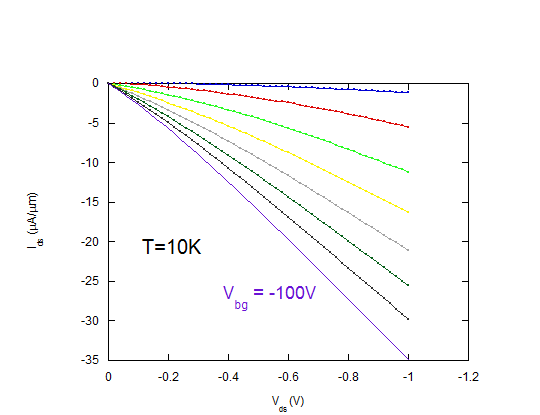
\includegraphics[height=4.55cm,width=5.3cm]{figs/results/hall_bar_doped_channel_doped_contacts/Vds-Id_Vds_1V_-1V-Vbg_-30V_-100V_T2-T3_10K-03_plot_before_anneal_5-5_21_no1}
		\label{fig:5-5_21_no1_pre_anneal_iv_10k}
	}
	\subfloat[]{
		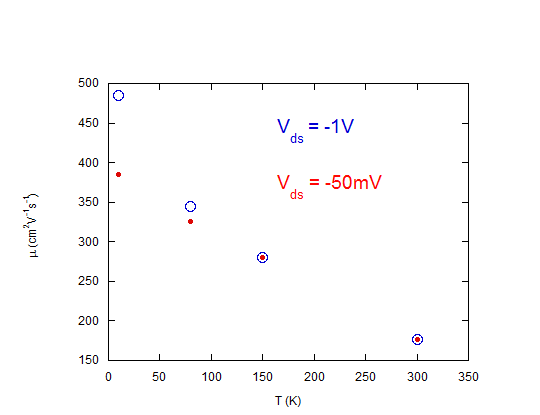
\includegraphics[height=4.55cm,width=5.3cm]{figs/results/hall_bar_doped_channel_doped_contacts/Two_Probe_FE_Mobility_Vs_T_Vds_-1V_-50mV_plot_pre_anneal_5-5_21_no1}
		\label{fig:5-5_21_no1_pre_anneal_mu_fe_vs_temp}
	}
	\caption[Characteristics of \ch{WSe2} \acs{FET} with lightly $p$-doped channel and 2D/2D contacts: I]{\protect\subref{fig:5-5_21_no1_pre_anneal_iv_300k} $IV$ chacteristics of device at $T=300\unita{K}$ and \protect\subref{fig:5-5_21_no1_pre_anneal_iv_10k} at $T=10\unita{K}$. \protect\subref{fig:5-5_21_no1_pre_anneal_mu_fe_vs_temp} Two-terminal field-effect mobility as a function of temperature for $V_{ds}=-50\unita{mV}$ and $-1\unita{V}$. \emph{Note: figures correspond to device shown in fig.~\subref*{fig:pWSe2_doped_contacts_and_channel_final_device}. Measurements shown were made before the device was annealed}.}
	\label{fig:pre_anneal_mu_fe_measurements}
\end{figure}
In an effort to improve the device's properties, the device was annealed for 30 minutes at $250^\degree\unita{C}$. During the process of annealing some of the organic matter that is affecting the device at lower temperatures is hoped to be removed and thus improving the device's performance \cite{Britton_NanoLett2013}. 
\begin{figure}[ht]
	\centering
	\subfloat[]{
		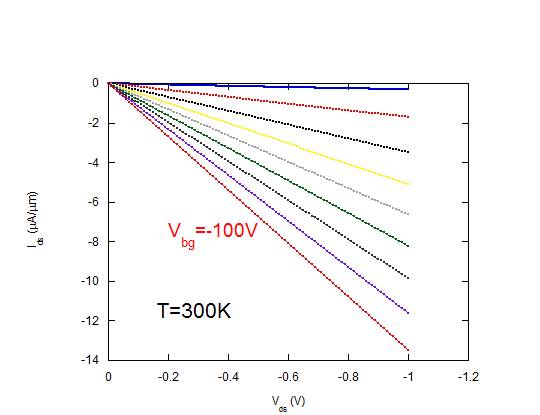
\includegraphics[height=4.55cm,width=5.3cm]{figs/results/hall_bar_doped_channel_doped_contacts/Vds-Id_Vds_1V_-1V-Vbg_-20V_-100V_T2-T3_300K-13_plot_after_anneal_5-5_21_no1}
		\label{fig:5-5_21_no1_post_anneal_iv_300k}
	}
	\subfloat[]{
		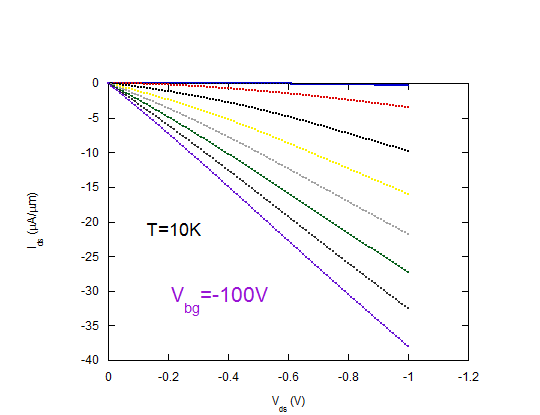
\includegraphics[height=4.55cm,width=5.3cm]{figs/results/hall_bar_doped_channel_doped_contacts/Vds-Id_Vds_1V_-1V-Vbg_-30V_-100V_T2-T3_10K-03_plot_after_anneal_5-5_21_no1}
		\label{fig:5-5_21_no1_post_anneal_iv_10k}
	}
	\subfloat[]{
		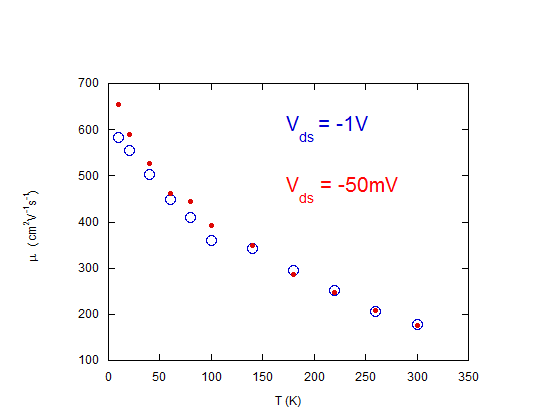
\includegraphics[height=4.55cm,width=5.3cm]{figs/results/hall_bar_doped_channel_doped_contacts/Two_Probe_FE_Mobility_Vs_T_Vds_-1V_-50mV_plot_post_anneal_5-5_21_no1}
		\label{fig:5-5_21_no1_post_anneal_mu_fe_vs_temp}
	}
	\caption[Characteristics of \ch{WSe2} \acs{FET} with lightly $p$-doped channel and 2D/2D contacts: II]{\protect\subref{fig:5-5_21_no1_post_anneal_iv_300k} $IV$ chacteristics of device at $T=300\unita{K}$ and \protect\subref{fig:5-5_21_no1_post_anneal_iv_10k} at $T=10\unita{K}$. \protect\subref{fig:5-5_21_no1_post_anneal_mu_fe_vs_temp} Two-terminal field-effect mobility as a function of temperature for $V_{ds}=-50\unita{mV}$ and $-1\unita{V}$. \emph{Note: figures correspond to device shown in fig.~\subref*{fig:pWSe2_doped_contacts_and_channel_final_device}. Measurements shown were made after the device was annealed for 30 minutes at $250^\degree\unita{C}$}.}
	\label{fig:post_anneal_mu_fe_measurements}
\end{figure}
Figs.~\ref{fig:5-5_21_no1_post_anneal_iv_300k} and \ref{fig:5-5_21_no1_pre_anneal_iv_10k} show the $IV$ characteristic curves for the device after it has been annealed. It shows the previously observed ohmic behavior at high temperature, while it also shows a corrected behavior at low temperature with less delineated behavior. As a result, in fig.~\ref{fig:5-5_21_no1_post_anneal_mu_fe_vs_temp} one observes slightly improved mobility values at lower temperatures and there is no longer a deviation at low temperature for the two $V_{ds}$ values. 

\subsection{Applying Low-Resistance Contacts: Undoped Channel}\label{subsec:mufe_undoped_channel}
In addition to determining how the doping of channel material affects its properties, the contact method from sec.~\ref{sec:contacts} was also applied to an undoped channel to determine its field-effect mobility and how well the new contact method can improve the performance. Using the same method as was for the doped channel (\lightlyone) device in subsec.~\ref{subsec:mufe_doped_channel} using a \hbn substrate and degenerately doped (\degenerate) contacts with a \hbn cover and a few-layer, undoped \ch{WSe2} channel as shown in fig.~\ref{fig:undoped_wse2_pic}. The quality of the contacts for the device are appartent in the inset of fig.~\ref{fig:undoped_wse2_mu_fe} as the $IV$ curves are linear at $T=5\unita{K}$. The conductivity as a function of backgate voltage $V_{bg}$ is pictured in fig.~\ref{fig:undoped_wse2_conduct} for various temperatures. It shows results consistent with expectation, the mobility increases with $V_{bg}$ and mobility also increases with decreasing temperature. Furthermore, the filed-effect mobility is shown in fig.~\ref{fig:undoped_wse2_mu_fe} showing increasing mobility with decreasing temperature, consistent with expectation. 
\begin{figure}[ht]
	\centering
	\subfloat[]{
		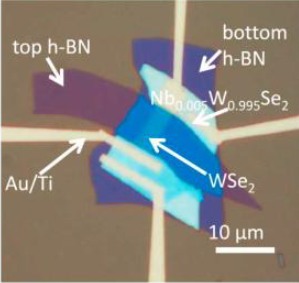
\includegraphics[height=4.5cm,width=5cm]{figs/results/ben/undoped_wse2_degen_doped_contacts}
		\label{fig:undoped_wse2_pic}
	}
	\subfloat[]{
		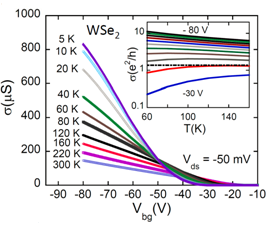
\includegraphics[height=4.5cm,width=5cm]{figs/results/ben/conductivity_2d2d_contacts_vs_Vbg_wse2}
		\label{fig:undoped_wse2_conduct}
	}
	\subfloat[]{
		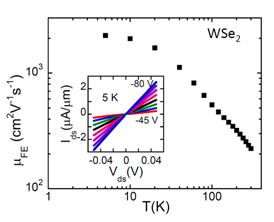
\includegraphics[height=4.5cm,width=5cm]{figs/results/ben/mu_fe_2d2d_contacts_vs_T_wse2}
		\label{fig:undoped_wse2_mu_fe}
	}
	\caption[Characteristics and channel properties of \ch{WSe2} \acs{FET} with 2D/2D contacts]{\protect\subref{fig:undoped_wse2_pic} Optical micrograph of \ch{WSe2} \acs{FET} with degenerately $p$-doped \ch{WSe2} (\degenerate) contacts with channel region on \hbn substrate and covered with a top \hbn piece. \protect\subref{fig:undoped_wse2_conduct} Temperature dependent two-terminal conductivity as a function of $V_{bg}$ at $V_{ds}=-50\unita{mV}$ for device shown in \protect\subref{fig:undoped_wse2_pic}. \protect\subref{fig:undoped_wse2_mu_fe} Two-terminal field-effect mobility. Figures appeared in ref.~\cite{Chuang_2016}.}
	\label{fig:mu_fe_data_degenerate}
\end{figure}

\subsection{Discussion of Two-Probe Measurement Results in Doped and Undoped Channels}\label{subsec:discussion_two_probe}
The results of field-effect mobility measurements using a lightly doped (\lightlyone) channel with degenerately doped channel show a $T=300\unita{K}$ field-effect mobility $\mu_\mathrm{FE}=180\cmvs$. This value is on the same order of magnitude as previously measured results using $p$-doped, few-layer \ch{WSe2} device. Pradhan \emph{et al.} reported a maximum mobility of $\mu_\mathrm{FE}=350\cmvs$ at the same temperature. In addition, the low temperature mobilities are also consistent with previous results where $\mu_\mathrm{FE}=650\cmvs$ at $T=150\unita{K}$ compared to our $\mu_\mathrm{FE}=350\cmvs$ at the same temperature \cite{Pradhan_SciReports2015}. The mobility measurements show that, in general, the mobility at high temperatures is dominated by phonon scattering \cite{Ando_RevModPhys1982}. This effect is diminished as the temperature is increased and the scattering becomes primarily due to Coulomb scattering and impurities. Therefore, one can deduce that by changin the doping content of the channel coupled with the use of the new contact method mobility can be tuned with the right approach, which is useful when it comes to applications. The ability to demonstrate low-resistance 2D/2D contacts is important. It enables the investigation of the intrinsic channel properties of the device, namely how the scattering mechanisms effect the mobility. A better understanding of how these mechanisms work leads to a further understanding of how the device performance can be improved.

\section{Hall Effect and Applying Low-Resistance Contacts}\label{sec:hall_effect_intro}
The field-effect mobility $\mu_\mathrm{FE}$ is one quantity to characterize the quality of a device. Another widely used quantity is the Hall mobility $\mu_H$. The Hall mobility is measured using the Hall effect. This quantity is useful because it directly gives several values that are not readily calcuable from using the field-effect mobility, such as resistivity $\rho$, mobility $\mu$, and (charge) carrier density $n$ \cite{Schroder_Semiconductor2006}. Consider the setup shown in fig.~\ref{fig:hall_diagram}, where $L$ is taken to be in the $x$-direction, width $w$ in the $y$-direction, thickness $t$ in the $z$-direction, and $e$ denotes a charge carrier which can either be an electron or a hole. The current $I$ flows in the positive $x$-direction and is given by
\begin{equation}\label{eq:current}
	I = J w t = n e v_x w t,
\end{equation}
where $J$ is the current density in the $x$-direction, $n$ is the charge carrier number density, and $v_x$ is the charge carrier drift velocity in the positive $x$-direction. The current $I$ is a result of the application of an electric field $E_x$ along the positive $x$-direction. In the presence of a magnetic field $B$ applied in the positive $z$-direction the charge carrier will experience a Lorentz for that deflects them towards one side of the device. As a result there is an accumulation of charges along one side of the device which in turn creates a transverse electric field $E_y$ \cite{Melissinos_Experiments1966}. This transverse electric field is given by
\begin{equation}\label{eq:Ey}
	E_y = v_x B.
\end{equation}
The accumulation of charges on one side of the device creates a potential differnece that is related to the this transverse electric field and be used to find the Hall voltage $V_H$ by integrating across the width of the device to arrive at
\begin{equation}\label{eq:V_H}
	V_H = -\frac{IB}{t}\left(\frac{1}{ne}\right).
\end{equation}
From eq.~\ref{eq:RH} the Hall coefficient is found to be
\begin{equation}\label{eq:RH}
	R_H = \frac{1}{ne} = \frac{V_H t}{IB}.
\end{equation}
Since $e$ refers to either electrons or holes, the sign of $R_H$ would also vary in accord with the proper carrier being described in the given circumstance. Furthermore, the conductivity is given by
\begin{equation}\label{eq:sigma}
	\sigma = n e \mu_H,
\end{equation}
where $\sigma$ is the conductivity and $\mu_H$ denotes the Hall mobility. Thus, an expression for the Hall mobility can be found by combining eqs.~\ref{eq:RH} and \ref{eq:sigma} to give
\begin{equation}\label{eq:mu_H}
	\mu_H = \abs{R_H}\sigma = \frac{\sigma V_H t}{IB}.
\end{equation}
As stated above, the result from eqs.~\ref{eq:RH} and \ref{eq:mu_H} give a direct relation using measurable and calcuable quantities to the carrier density, resistivity ($\rho=\sigma^{-1}$), and the hall mobility. Using this method, one can further characterize a device's behavior to better understand the mechanisms that control and limit the performance at high and low temperatures as well as the effects of doping the channel, and how this information can be used to further improve the performance of the device.
\begin{figure}[ht]
	\centering
	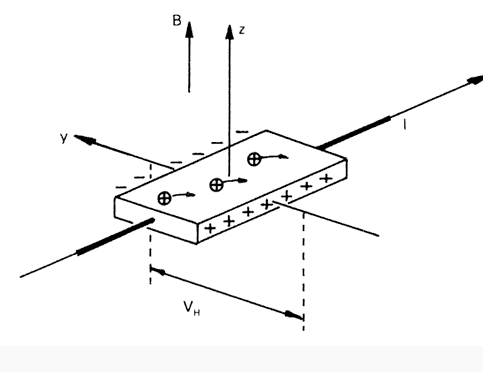
\includegraphics[height=6cm,width=8cm]{figs/results/hall_diagram}
	\caption[Hall effect measurement diagram]{Geometry of Hall effect measurement. Current flows in the positive $x$-direction and magnetic field is applied in the positive $z$ direction generating a Hall voltage \cite{HallEffectNIST}. Diagram originally appeared in ref.~\cite{HallDiagram}.}
	\label{fig:hall_diagram}
\end{figure}

\subsection{Hall Effect: \lightlyfive}\label{subsec:hall_lightly}
In order to perform the Hall measurement the device design is important. There need to be electrodes that are properly aligned parallel to one another in order to measure the longitudinal conductance (resistivity $\rho_{xx}=\sigma_{xx}^{-1}$) $\sigma_{xx}$ and the transverse conductivity (resistivity $\rho_{xy}=\sigma_{xy}^{-1}$) $\sigma_{xy}$ (the conductivity used to measure the Hall mobility). Fig.~\ref{fig:hall_bar_device1} shows an optical micrograph of the design used for the Hall measurement in this case. Note that the channel material used here was lightly doped \ch{WSe2} ($\lightlyfive$). Fig.~\subref*{fig:11192015_ohmic_contacts} shows the $IV$ characteristic curve of the device as a function of $V_{ds}$ for several backgate voltages at $T=300\unita{K}$. This shows that the device exhibits linear and ohmic contacts at this temperature. Fig.~\subref*{fig:11192015_conduct_vs_temp} shows the conductivity $\sigma$ as a function of backgate voltage $V_{bg}$ for various temperatures. The trend shown, conductivity increasing as temperature increases for the same $V_{bg}$, is not what is expected to occur. Instead, the conductivity should increase with decreasing temperature. The fact that this device exhibits this behavior points to the development of some barrier that degrades the device's performance.  
\begin{figure}[ht]
	\centering
	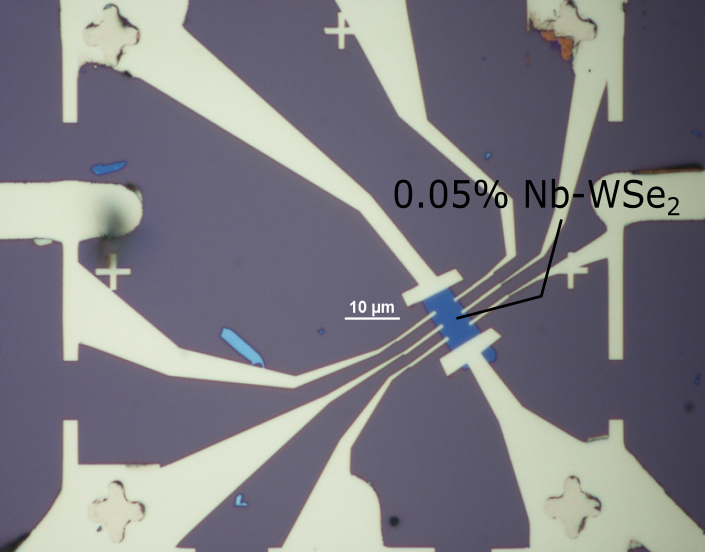
\includegraphics[height=4.5cm,width=6.0cm]{figs/results/hall_bar_doped_channel/hall_bar_device_pic_11192015_no2_doping_scheme}
	\caption[Hall bar device optical micrograph using \lightlyfive]{Optical micrograph of device structure consisting of lightly $p$-doped \ch{WSe2} (\lightlyfive) with device thickness $7.7\unita{nm}$ and \ch{Ti}/\ch{Au} metal contacts.}
	\label{fig:hall_bar_device1}
\end{figure}
This is further confirmed in fig.~\subref*{fig:11192015_mu_hall_vs_temp} where the Hall mobility $\mu_H$ as a function of $V_{bg}$ for various temperatures is shown. Again, one would expect that as temperature is increased, the mobility would decrease. However, the reserve is true in this device. There are several reasons for this. Phonon scattering can be ruled out as a cause, because that is primarily temperature dependent and its effect would decrease with decreasing temperature raising the mobility. Therefore, the resulting degradation of mobility here are due to Coulomb scattering, surface and roughness scattering, and impurities introduced from doping the channel and the lack of a \hbn channel cover.
\begin{figure}[ht]
	\centering
	\subfloat[]{
		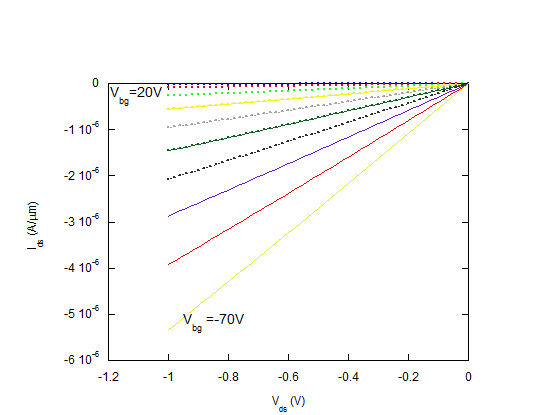
\includegraphics[height=4.25cm,width=5.0cm]{figs/results/hall_bar_doped_channel/Vds-Id_1V_-1V-Vbg_20V_-70V_T1-D_T5_S_300K_plot_modified_11192015_no2}
		\label{fig:11192015_ohmic_contacts}
	}
	%\qquad
	\subfloat[]{
		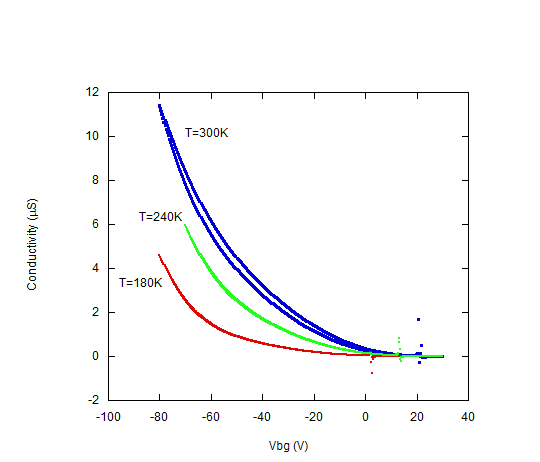
\includegraphics[height=4.25cm,width=5.0cm]{figs/results/hall_bar_doped_channel/hall_bar_device_pic_11192015_no1_conduct_vs_Vbg_all_temps}
		\label{fig:11192015_conduct_vs_temp}
	}
	\subfloat[]{
		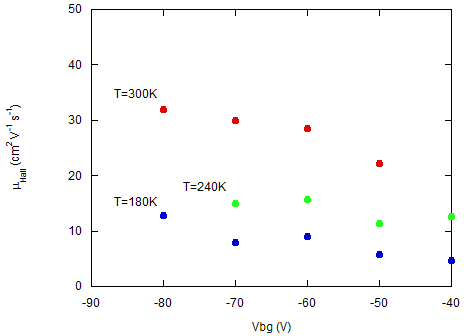
\includegraphics[height=4.25cm,width=5.0cm]{figs/results/hall_bar_doped_channel/hall_bar_device_pic_11192015_no1_mu_hall_vs_Vbg_all_temps}
		\label{fig:11192015_mu_hall_vs_temp}
	}

	%\qquad
	\subfloat[]{
		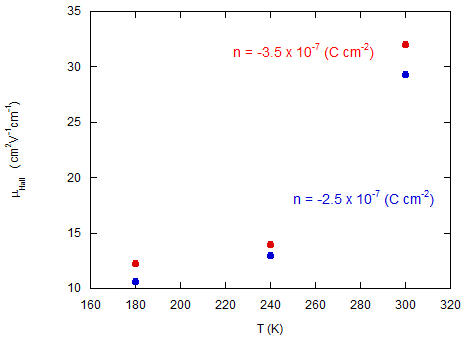
\includegraphics[height=4.25cm,width=5.0cm]{figs/results/hall_bar_doped_channel/HallMobility_Vs_T_for_fixed_carrier_consentrations_plot_modified_11192015_no2}
		\label{fig:11192015_mu_hall_vs_temp_various_n}
	}
	\qquad
	\subfloat[]{
		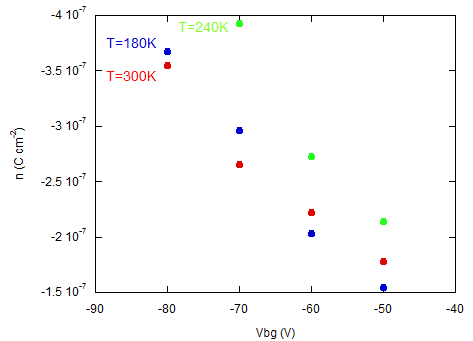
\includegraphics[height=4.25cm,width=5.0cm]{figs/results/hall_bar_doped_channel/Charge_density_Vs_Vbg_different_Temp_plot_modified_11192015_no1}
		\label{fig:11192015_n_vs_Vbg}
	}
	\caption[Output characteristics and channel properties of lightly $p$-doped \ch{WSe2} with 2D/2D contacts]{\protect\subref{fig:11192015_ohmic_contacts} $IV$ characteristic curve at $T=300\unita{K}$ as a function of $V_{ds}$ for $V_{bg}$ ranging from $-70\unita{V}$ to $20\unita{V}$. \protect\subref{fig:11192015_conduct_vs_temp} Temperature-dependence of conductivity and \protect\subref{fig:11192015_mu_hall_vs_temp} Hall mobility as a function of $V_{bg}$. \protect\subref{fig:11192015_mu_hall_vs_temp_various_n} Charge carrier denisty dependence of Hall mobility as a function of temperature and \protect\subref{fig:11192015_n_vs_Vbg} temperature dependence of charge carrier density as a function of $V_{bg}$. \emph{Note: the data here corresponds to device shown in fig.~\ref{fig:hall_bar_device1}}.}
	\label{fig:hall_measurement_data_lightly}
\end{figure}
Fig.~\subref*{fig:11192015_mu_hall_vs_temp_various_n} illustrates the Hall mobility as a function of charge carrier densities $n=-3.5\times 10^{-7}\unita{C}\unitb{cm}{-2}$ and $n=-2.5\times 10^{-7}\unita{C}\unitb{cm}{-2}$. As charge carrier density is increased through the increase of $V_{bg}$ the mobility increases due to more the introduction of more carriers. In addition, in principle one would expect that for a given $V_{bg}$ the carrier density should be the same across all temperatures. More specifcally, fig.~\subref*{fig:11192015_n_vs_Vbg} should show the points all along the same line, however, there is some discrepancy. The slope of this curve would give the capacitance and the expectation is that the value would be the same within some relative error, but the lack of this fact points to some device defects that need to further improved upon.

\subsection{Hall Effect: Discussion and Improvements}\label{subsec:hall_improvements}
The Hall mobilities reported using this lightly doped (\lightlyfive) device range from $\mu_H=31.9\cmvs$ at $T=300\unita{K}$ to $\mu_H=16.7\cmvs$ at $T=180\unita{K}$. Compared to literature values for few-layer $p$-type \ch{WSe2} Hall mobilities, these values are an order of magnitude lower \cite{Pradhan_SciReports2015}. Several improvements, however, can be made to the device fabrication that can readily improve the observed mobility. First, the use of a \hbn substrate instead of \ch{Si}/\ch{SiO2} substrate would reduce the likelyhood of scattering due to roughness and interface effects between it and the channel. Second, the use of a \hbn cover over the channel would also decrease any external effects and protect the channel. Finally, and most importantly, applying the 2D/2D contact method would improve the mobility of the device across all temperatures. \\ \\
In addition to using the doped channel material, with the use of the 2D/2D contact method, it is hopeful to reach high-quality devices in the bilayer and multilayer regimes. Previously measured results have shown other \acp{TMD} can achieve high mobilities reaching $34,000\cmvs$ using graphene contacts \cite{Li_NatureNano2015}. For reasons stated before in sec.~\ref{sec:contacts} this is not viable for \ch{WSe2}. This goal in both $p$ and $n$-type \ch{WSe2} is desired because it would ultimately lead to the ability to study the quantum transport properties that are not readily attainable with device's of lesser quality. However, this poses many challenges such as fabricating devices that have high mobilities ($>10^{3}\cmvs$) at low temperatures ($<4\unita{K}$).

%\begin{figure}[ht]
%	\centering
%	\subfloat[]{
%		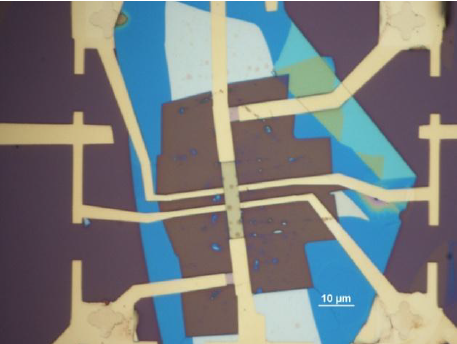
\includegraphics[height=4.75cm,width=5.5cm]{figs/results/ben/pWSe2_hall}
%		\label{fig:pWSe2_hall}
%	}
%	\qquad
%	\subfloat[]{
%		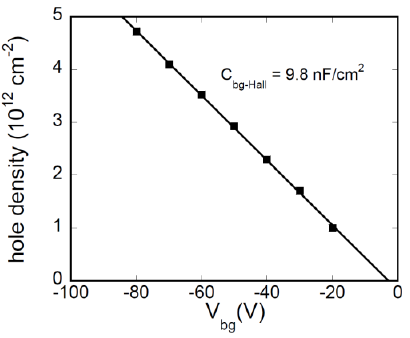
\includegraphics[height=4.75cm,width=5.5cm]{figs/results/ben/pWSe2_cap}
%		\label{fig:pWSe2_cap}
%	}
%	\caption[Hall effect measurement with 2D/2D contacts to determine capacitance]{\protect\subref{fig:pWSe2_hall} Optical microgrpah of \ch{WSe2} Hall bar device encapsulated in \hbn with degenerate 2D/2D contacts. \protect\subref{fig:pWSe2_cap} Hole density as a function of $V_{bg}$ at $T=300\unita{K}$ extracted from Hall effect measurement. Figures appeared in ref.~\cite{Chuang_2016}.}
%	\label{fig:pWSe2_hall_ben}
%\end{figure}